\section{Inclusion of SRF wings}
%===============================
\label{app:Rset}
This appendix contains the comparisons of low and effective high spectral resolution digitized SRFs for the nominal (20\textdegree{}C) baseplate temperature and bias voltage (Vnom) from the ATMS PFM Calibration Data Book\cite{ATMS_PFM_CalLog}. The low spectral resolution data includes the SRF ``wings'' seen for insertion losses as large as -40dB - an example for channel 1 is shown in figure \ref{fig:ch1.RESlow}. The high spectral resolution data concentrates on the central peak of the SRF to precisely locate the -3dB level (roughly equivalent to the half-power point) - an example for the same channel 1 measurement is shown in figure \ref{fig:ch1.REShi}.

To determine the impact of including the SRF wings in the brightess temperature calculations, rather than use the actual high spectral resolution digitized SRFs, a truncated dataset was created where the low spectral resolution SRFs were cutoff at the -10dB level (equivalent to a relative response of 0.1). This ensures any $T_B$ differences are due to the SRF wings, not to digitization errors, normalization differences, etc. Note, however, that no assumption has been made about any frequency rejection of the signal in the instrument electronics (as intimated by the listing of the lower and upper rejection points in figure \ref{fig:ch1.RESlow}). The digitizations used for this analysis were performed by Lynn Chidester of the Space Dynamics Laboratory (SDL) at Utah State University. Included in the SRF plots are the ``boxcar'' SRF, based on the table \ref{tab:atms_fo_sb_and_df} data, and a representative brightness temperature spectrum.

Shown alongside each SRF comparison are the brightness temperature differences for the SRFs with respect to the boxcar response. MonoRTM \cite{Clough_2005} was used to compute the top-of-atmosphere brightness temperatures for the ECMWF83 profile data set \cite{ECMWF_profile_set2,Matricardi_ECMWF564} at the frequencies of the SRFs. These monochromatic brightness temperatures were then integrated over frequency to provide the channel brightness temperatures.

\newpage
 
\begin{figure}[H]
  \centering
  \includegraphics[bb=368 260 1540 1062,scale=0.25]{graphics/srf/Rset/ch1.RESlow.eps}
  \caption{Example of plot of low spectral resolution SRF display in the ATMS PFM Calibration Data Book\cite{ATMS_PFM_CalLog}.}
  \label{fig:ch1.RESlow}
\end{figure}

\begin{figure}[H]
  \centering
  \includegraphics[bb=368 260 1540 1062,scale=0.25]{graphics/srf/Rset/ch1.REShi.eps}
  \caption{Example of plot of high spectral resolution SRF display in the ATMS PFM Calibration Data Book\cite{ATMS_PFM_CalLog}.}
  \label{fig:ch1.REShi}
\end{figure}

\newpage
 
\begin{figure}[H]
  \centering
  \begin{tabular}{c c c}
    \textsf{\textbf{(a)} SRFs} &
    \textsf{\textbf{(b)} $\Delta T_B$ $(\epsilon_s = 1.0)$} &
    \textsf{\textbf{(c)} $\Delta T_B$ $(\epsilon_s = 0.6)$} \\
    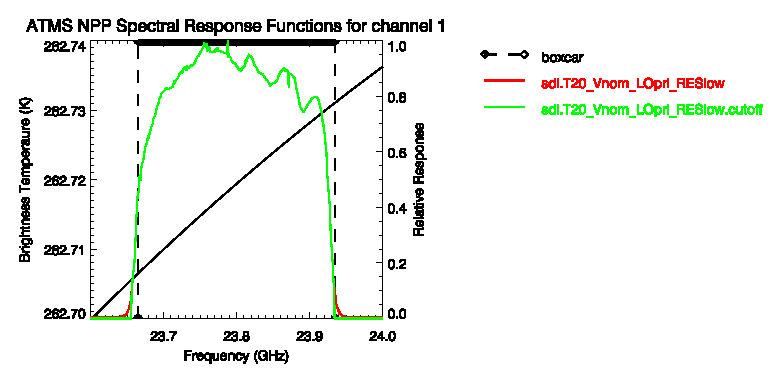
\includegraphics[bb=80 400 280 558,clip,scale=0.85]{graphics/srf/Rset/atms_npp.ch1.osrf.eps} &
    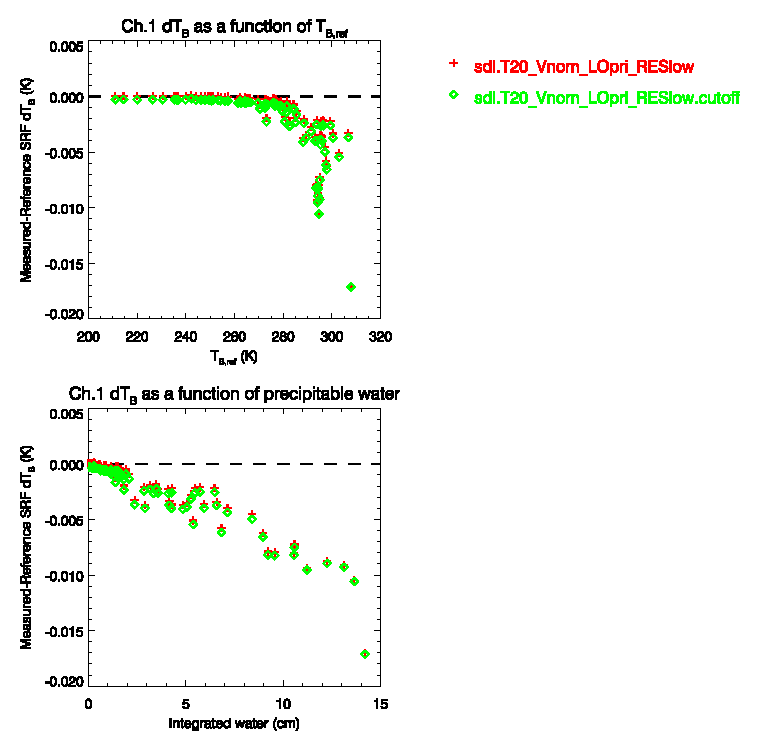
\includegraphics[bb=85 400 260 558,clip,scale=0.85]{graphics/dtb/Rset/e1.0_r0.0/atms_npp.ch1.dTb.eps} & 
    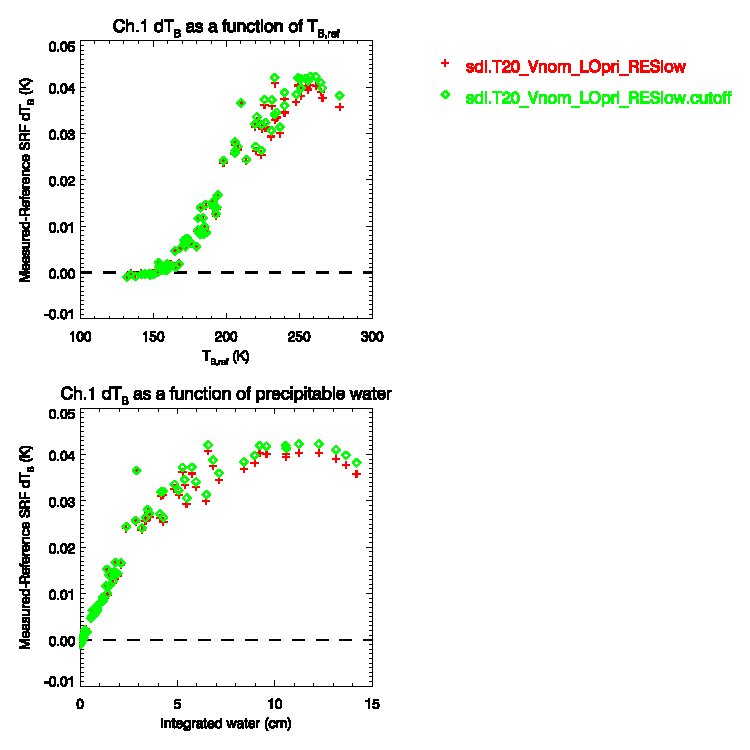
\includegraphics[bb=85 400 290 558,clip,scale=0.85]{graphics/dtb/Rset/e0.6_r0.4/atms_npp.ch1.dTb.eps} 
  \end{tabular} \\
  % the hand-crafted legend
  \setlength{\unitlength}{1cm}
  \begin{picture}(8.0,1.0)
    \thicklines
    \color{red}
    \put(-0.5,0.5){\line(1,0){1}}
    \put(0.7,0.35){\sffamily \textbf{+}\quad SRF wings included}
    \color{green}
    \put(5.0,0.5){\line(1,0){1}}
    \put(6.2,0.35){\sffamily {\Large$\diamond$}\quad SRF cutoff at -10dB}
  \end{picture}
  \caption{Channel 1 NPP ATMS nominal baseplate temperature (20\textdegree{}C) and bias voltage \textbf{(a)} SRF data digitized from the low spectral resolution plots in the ATMS PFM Calibration Data Book\cite{ATMS_PFM_CalLog} along with an SRF truncated at -10dB. The corresponding boxcar response based on table \ref{tab:atms_fo_sb_and_df} and a representative brightness temperature spectrum is also shown. \textbf{(b)} Brightness temperature differences showing the impact of excluding the SRF wings beyong -10dB, derived from MonoRTM calculations with a surface emissivity of unity. \textbf{(c)} Same as (b), but for surface emissivity and reflectivity of 0.6 and 0.4 respectively.}
  \label{fig:atms_npp.Rset.ch1}
\end{figure}
 
\begin{figure}[H]
  \centering
  \begin{tabular}{c c c}
    \textsf{\textbf{(a)} SRFs} &
    \textsf{\textbf{(b)} $\Delta T_B$ $(\epsilon_s = 1.0)$} &
    \textsf{\textbf{(c)} $\Delta T_B$ $(\epsilon_s = 0.6)$} \\
    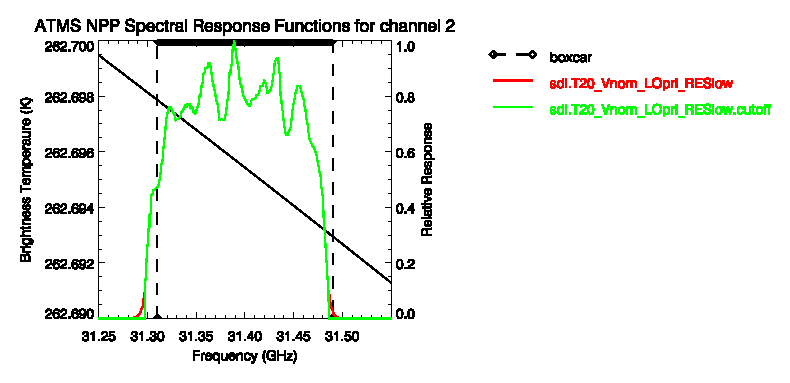
\includegraphics[bb=80 400 280 558,clip,scale=0.85]{graphics/srf/Rset/atms_npp.ch2.osrf.eps} &
    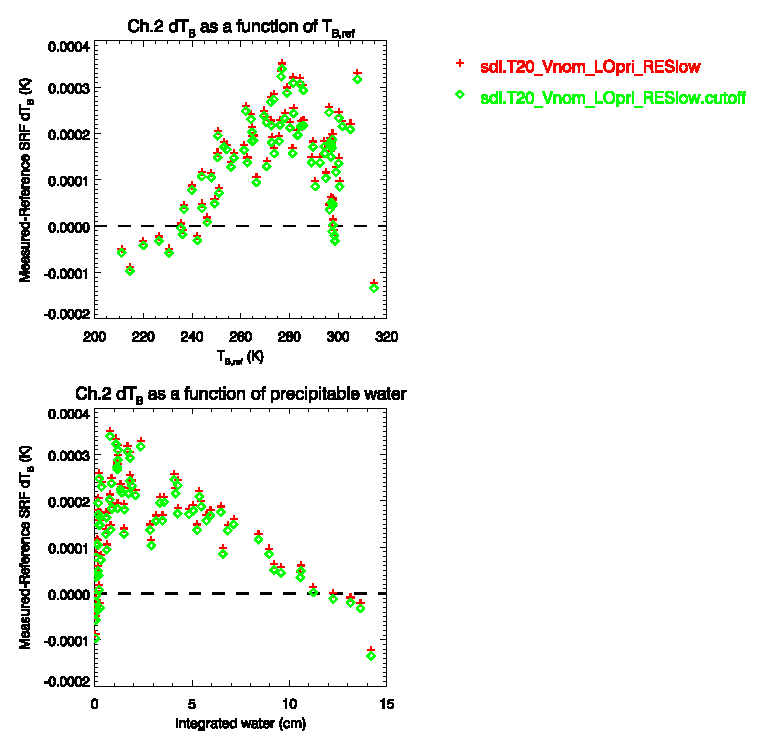
\includegraphics[bb=85 400 260 558,clip,scale=0.85]{graphics/dtb/Rset/e1.0_r0.0/atms_npp.ch2.dTb.eps} & 
    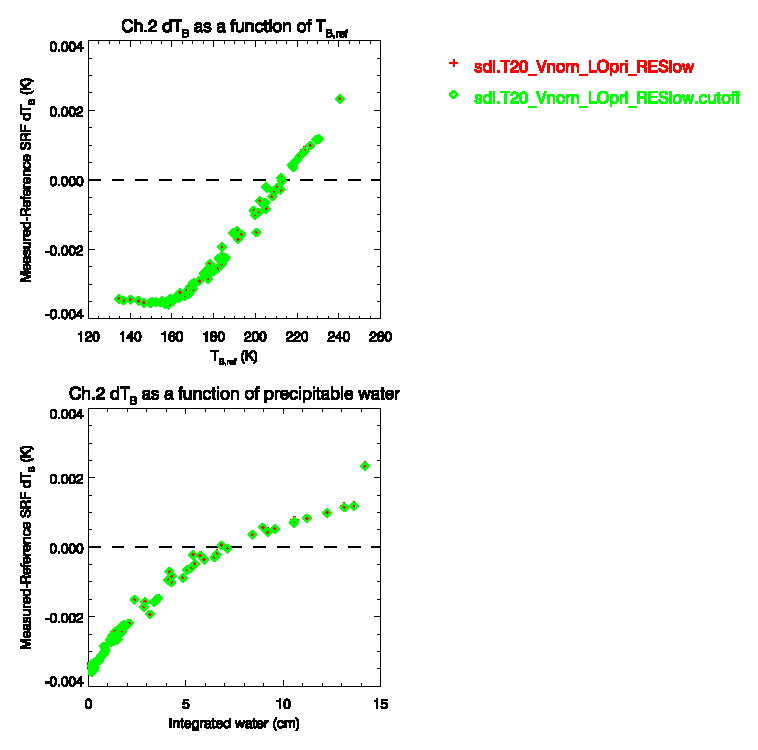
\includegraphics[bb=85 400 290 558,clip,scale=0.85]{graphics/dtb/Rset/e0.6_r0.4/atms_npp.ch2.dTb.eps} 
  \end{tabular} \\
  % the hand-crafted legend
  \setlength{\unitlength}{1cm}
  \begin{picture}(8.0,1.0)
    \thicklines
    \color{red}
    \put(-0.5,0.5){\line(1,0){1}}
    \put(0.7,0.35){\sffamily \textbf{+}\quad SRF wings included}
    \color{green}
    \put(5.0,0.5){\line(1,0){1}}
    \put(6.2,0.35){\sffamily {\Large$\diamond$}\quad SRF cutoff at -10dB}
  \end{picture}
  \caption{Channel 2 NPP ATMS nominal baseplate temperature (20\textdegree{}C) and bias voltage \textbf{(a)} SRF data digitized from the low spectral resolution plots in the ATMS PFM Calibration Data Book\cite{ATMS_PFM_CalLog} along with an SRF truncated at -10dB. The corresponding boxcar response based on table \ref{tab:atms_fo_sb_and_df} and a representative brightness temperature spectrum is also shown. \textbf{(b)} Brightness temperature differences showing the impact of excluding the SRF wings beyong -10dB, derived from MonoRTM calculations with a surface emissivity of unity. \textbf{(c)} Same as (b), but for surface emissivity and reflectivity of 0.6 and 0.4 respectively.}
  \label{fig:atms_npp.Rset.ch2}
\end{figure}
 
\begin{figure}[H]
  \centering
  \begin{tabular}{c c c}
    \textsf{\textbf{(a)} SRFs} &
    \textsf{\textbf{(b)} $\Delta T_B$ $(\epsilon_s = 1.0)$} &
    \textsf{\textbf{(c)} $\Delta T_B$ $(\epsilon_s = 0.6)$} \\
    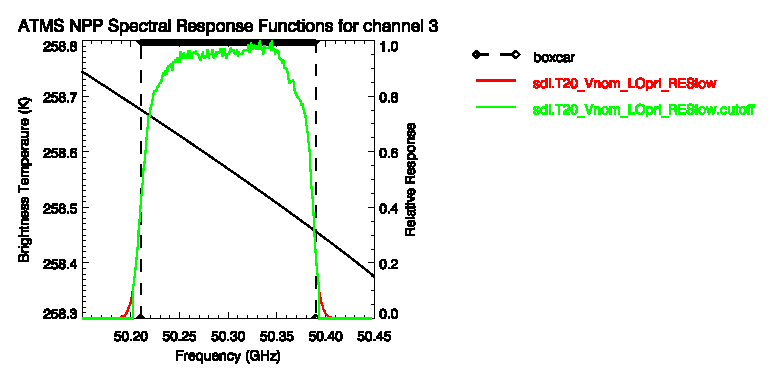
\includegraphics[bb=80 400 280 558,clip,scale=0.85]{graphics/srf/Rset/atms_npp.ch3.osrf.eps} &
    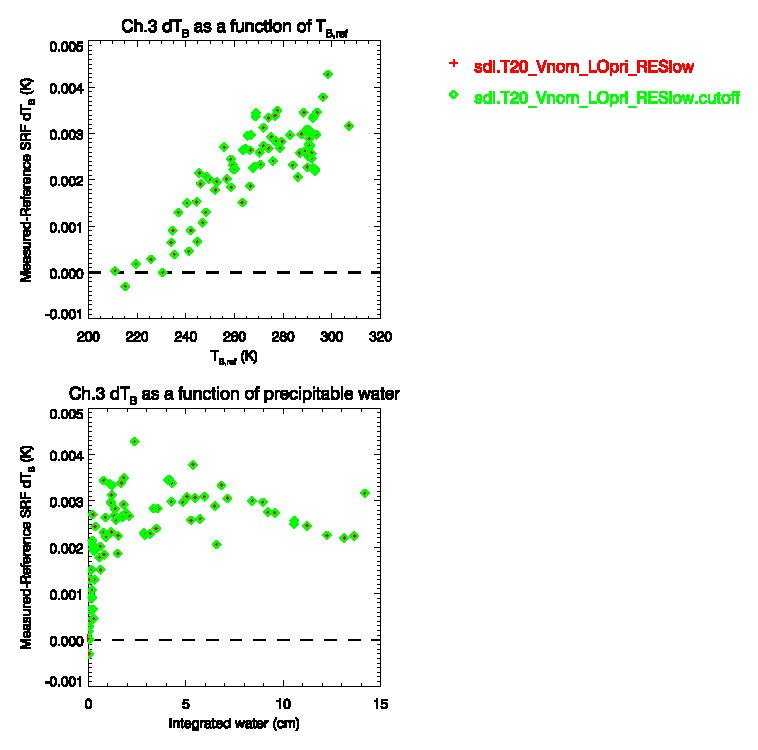
\includegraphics[bb=85 400 260 558,clip,scale=0.85]{graphics/dtb/Rset/e1.0_r0.0/atms_npp.ch3.dTb.eps} & 
    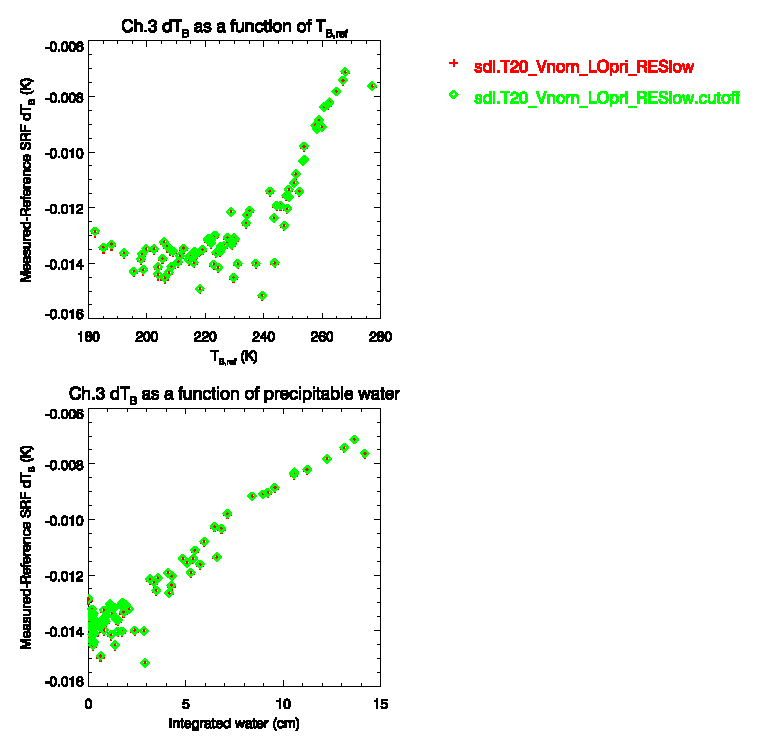
\includegraphics[bb=85 400 290 558,clip,scale=0.85]{graphics/dtb/Rset/e0.6_r0.4/atms_npp.ch3.dTb.eps} 
  \end{tabular} \\
  % the hand-crafted legend
  \setlength{\unitlength}{1cm}
  \begin{picture}(8.0,1.0)
    \thicklines
    \color{red}
    \put(-0.5,0.5){\line(1,0){1}}
    \put(0.7,0.35){\sffamily \textbf{+}\quad SRF wings included}
    \color{green}
    \put(5.0,0.5){\line(1,0){1}}
    \put(6.2,0.35){\sffamily {\Large$\diamond$}\quad SRF cutoff at -10dB}
  \end{picture}
  \caption{Channel 3 NPP ATMS nominal baseplate temperature (20\textdegree{}C) and bias voltage \textbf{(a)} SRF data digitized from the low spectral resolution plots in the ATMS PFM Calibration Data Book\cite{ATMS_PFM_CalLog} along with an SRF truncated at -10dB. The corresponding boxcar response based on table \ref{tab:atms_fo_sb_and_df} and a representative brightness temperature spectrum is also shown. \textbf{(b)} Brightness temperature differences showing the impact of excluding the SRF wings beyong -10dB, derived from MonoRTM calculations with a surface emissivity of unity. \textbf{(c)} Same as (b), but for surface emissivity and reflectivity of 0.6 and 0.4 respectively.}
  \label{fig:atms_npp.Rset.ch3}
\end{figure}
 
\begin{figure}[H]
  \centering
  \begin{tabular}{c c c}
    \textsf{\textbf{(a)} SRFs} &
    \textsf{\textbf{(b)} $\Delta T_B$ $(\epsilon_s = 1.0)$} &
    \textsf{\textbf{(c)} $\Delta T_B$ $(\epsilon_s = 0.6)$} \\
    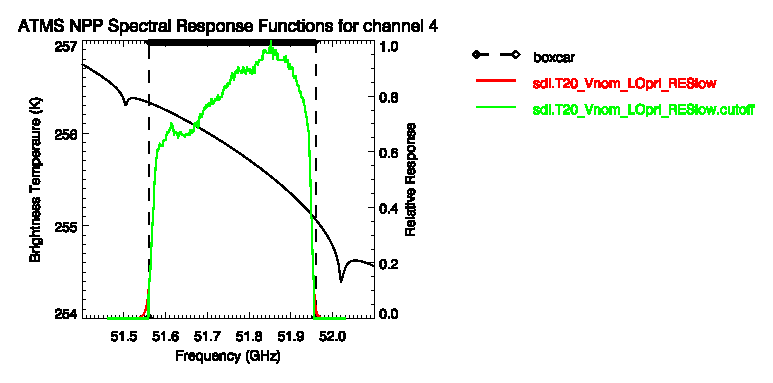
\includegraphics[bb=80 400 280 558,clip,scale=0.85]{graphics/srf/Rset/atms_npp.ch4.osrf.eps} &
    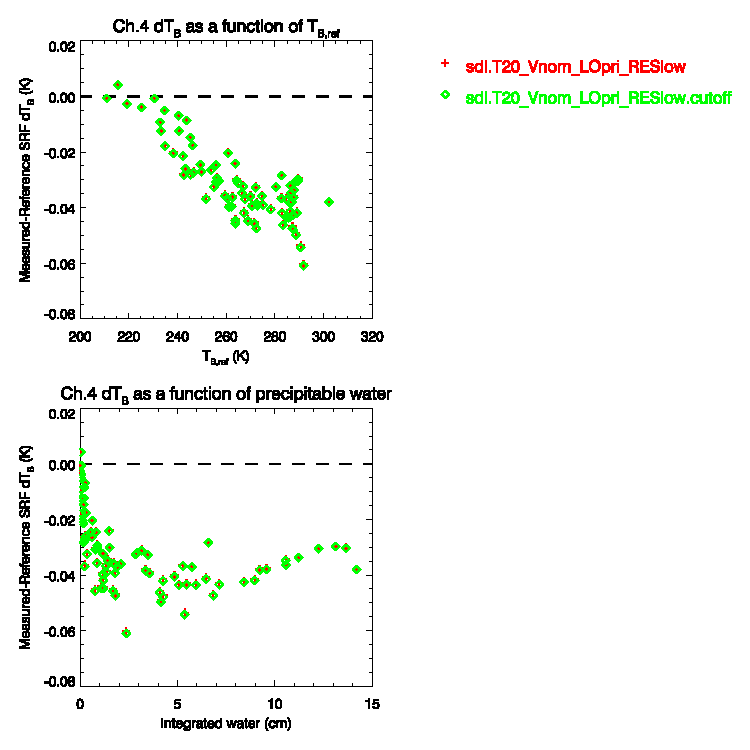
\includegraphics[bb=85 400 260 558,clip,scale=0.85]{graphics/dtb/Rset/e1.0_r0.0/atms_npp.ch4.dTb.eps} & 
    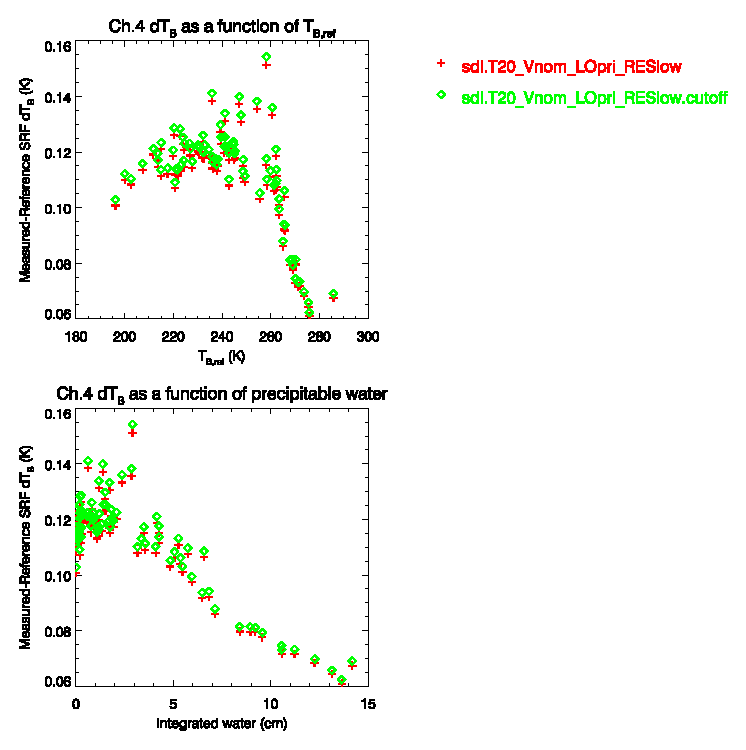
\includegraphics[bb=85 400 290 558,clip,scale=0.85]{graphics/dtb/Rset/e0.6_r0.4/atms_npp.ch4.dTb.eps} 
  \end{tabular} \\
  % the hand-crafted legend
  \setlength{\unitlength}{1cm}
  \begin{picture}(8.0,1.0)
    \thicklines
    \color{red}
    \put(-0.5,0.5){\line(1,0){1}}
    \put(0.7,0.35){\sffamily \textbf{+}\quad SRF wings included}
    \color{green}
    \put(5.0,0.5){\line(1,0){1}}
    \put(6.2,0.35){\sffamily {\Large$\diamond$}\quad SRF cutoff at -10dB}
  \end{picture}
  \caption{Channel 4 NPP ATMS nominal baseplate temperature (20\textdegree{}C) and bias voltage \textbf{(a)} SRF data digitized from the low spectral resolution plots in the ATMS PFM Calibration Data Book\cite{ATMS_PFM_CalLog} along with an SRF truncated at -10dB. The corresponding boxcar response based on table \ref{tab:atms_fo_sb_and_df} and a representative brightness temperature spectrum is also shown. \textbf{(b)} Brightness temperature differences showing the impact of excluding the SRF wings beyong -10dB, derived from MonoRTM calculations with a surface emissivity of unity. \textbf{(c)} Same as (b), but for surface emissivity and reflectivity of 0.6 and 0.4 respectively.}
  \label{fig:atms_npp.Rset.ch4}
\end{figure}
 
\begin{figure}[H]
  \centering
  \begin{tabular}{c c c}
    \textsf{\textbf{(a)} SRFs} &
    \textsf{\textbf{(b)} $\Delta T_B$ $(\epsilon_s = 1.0)$} &
    \textsf{\textbf{(c)} $\Delta T_B$ $(\epsilon_s = 0.6)$} \\
    \includegraphics[bb=80 400 280 558,clip,scale=0.85]{graphics/srf/Rset/atms_npp.ch5.osrf.eps} &
    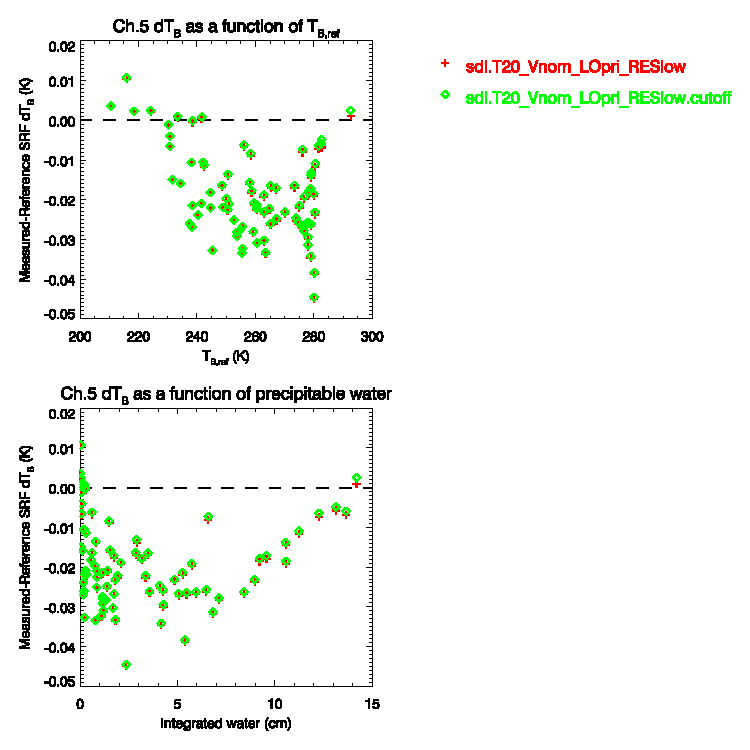
\includegraphics[bb=85 400 260 558,clip,scale=0.85]{graphics/dtb/Rset/e1.0_r0.0/atms_npp.ch5.dTb.eps} & 
    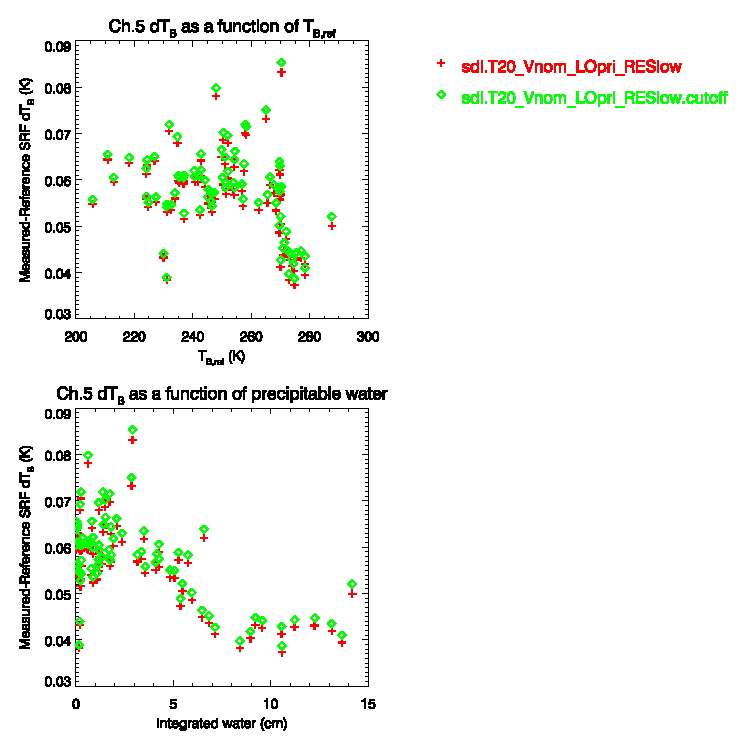
\includegraphics[bb=85 400 290 558,clip,scale=0.85]{graphics/dtb/Rset/e0.6_r0.4/atms_npp.ch5.dTb.eps} 
  \end{tabular} \\
  % the hand-crafted legend
  \setlength{\unitlength}{1cm}
  \begin{picture}(8.0,1.0)
    \thicklines
    \color{red}
    \put(-0.5,0.5){\line(1,0){1}}
    \put(0.7,0.35){\sffamily \textbf{+}\quad SRF wings included}
    \color{green}
    \put(5.0,0.5){\line(1,0){1}}
    \put(6.2,0.35){\sffamily {\Large$\diamond$}\quad SRF cutoff at -10dB}
  \end{picture}
  \caption{Channel 5 NPP ATMS nominal baseplate temperature (20\textdegree{}C) and bias voltage \textbf{(a)} SRF data digitized from the low spectral resolution plots in the ATMS PFM Calibration Data Book\cite{ATMS_PFM_CalLog} along with an SRF truncated at -10dB. The corresponding boxcar response based on table \ref{tab:atms_fo_sb_and_df} and a representative brightness temperature spectrum is also shown. \textbf{(b)} Brightness temperature differences showing the impact of excluding the SRF wings beyong -10dB, derived from MonoRTM calculations with a surface emissivity of unity. \textbf{(c)} Same as (b), but for surface emissivity and reflectivity of 0.6 and 0.4 respectively.}
  \label{fig:atms_npp.Rset.ch5}
\end{figure}
 
\begin{figure}[H]
  \centering
  \begin{tabular}{c c c}
    \textsf{\textbf{(a)} SRFs} &
    \textsf{\textbf{(b)} $\Delta T_B$ $(\epsilon_s = 1.0)$} &
    \textsf{\textbf{(c)} $\Delta T_B$ $(\epsilon_s = 0.6)$} \\
    \includegraphics[bb=80 400 280 558,clip,scale=0.85]{graphics/srf/Rset/atms_npp.ch6.osrf.eps} &
    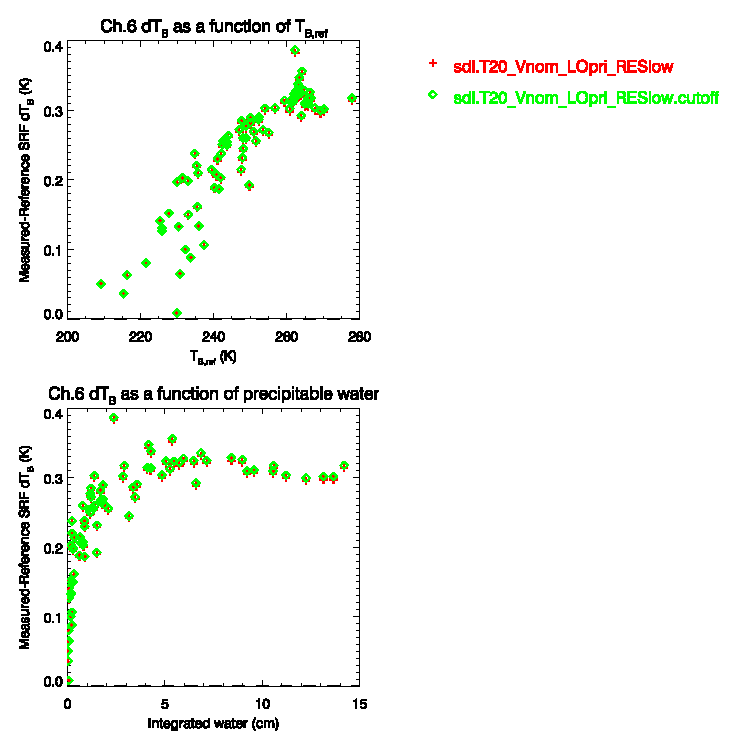
\includegraphics[bb=85 400 260 558,clip,scale=0.85]{graphics/dtb/Rset/e1.0_r0.0/atms_npp.ch6.dTb.eps} & 
    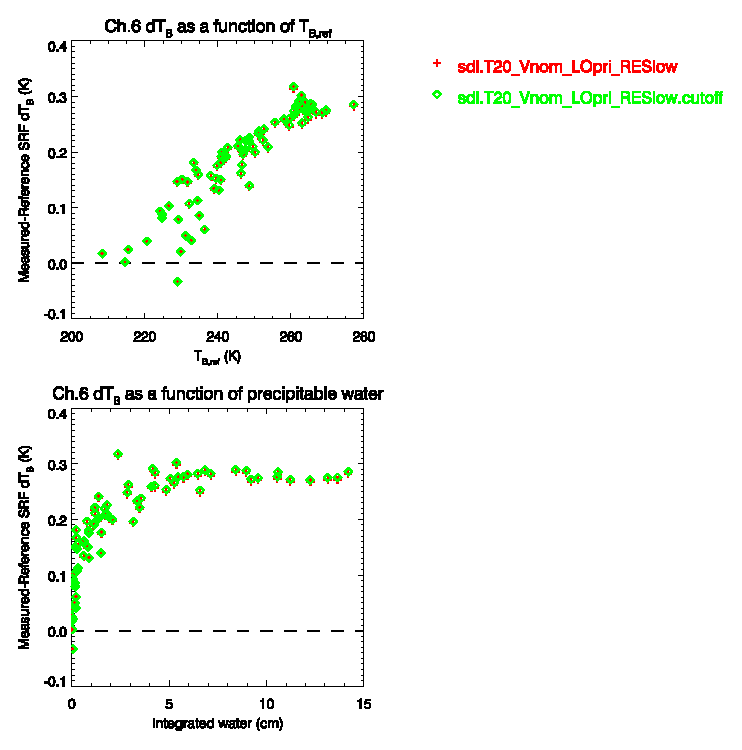
\includegraphics[bb=85 400 290 558,clip,scale=0.85]{graphics/dtb/Rset/e0.6_r0.4/atms_npp.ch6.dTb.eps} 
  \end{tabular} \\
  % the hand-crafted legend
  \setlength{\unitlength}{1cm}
  \begin{picture}(8.0,1.0)
    \thicklines
    \color{red}
    \put(-0.5,0.5){\line(1,0){1}}
    \put(0.7,0.35){\sffamily \textbf{+}\quad SRF wings included}
    \color{green}
    \put(5.0,0.5){\line(1,0){1}}
    \put(6.2,0.35){\sffamily {\Large$\diamond$}\quad SRF cutoff at -10dB}
  \end{picture}
  \caption{Channel 6 NPP ATMS nominal baseplate temperature (20\textdegree{}C) and bias voltage \textbf{(a)} SRF data digitized from the low spectral resolution plots in the ATMS PFM Calibration Data Book\cite{ATMS_PFM_CalLog} along with an SRF truncated at -10dB. The corresponding boxcar response based on table \ref{tab:atms_fo_sb_and_df} and a representative brightness temperature spectrum is also shown. \textbf{(b)} Brightness temperature differences showing the impact of excluding the SRF wings beyong -10dB, derived from MonoRTM calculations with a surface emissivity of unity. \textbf{(c)} Same as (b), but for surface emissivity and reflectivity of 0.6 and 0.4 respectively.}
  \label{fig:atms_npp.Rset.ch6}
\end{figure}
 
\begin{figure}[H]
  \centering
  \begin{tabular}{c c c}
    \textsf{\textbf{(a)} SRFs} &
    \textsf{\textbf{(b)} $\Delta T_B$ $(\epsilon_s = 1.0)$} &
    \textsf{\textbf{(c)} $\Delta T_B$ $(\epsilon_s = 0.6)$} \\
    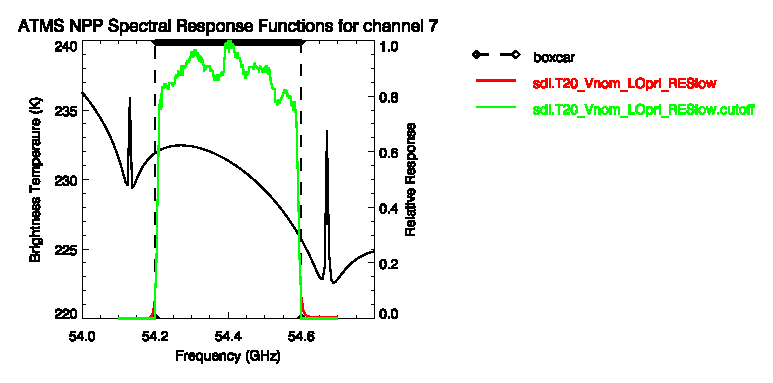
\includegraphics[bb=80 400 280 558,clip,scale=0.85]{graphics/srf/Rset/atms_npp.ch7.osrf.eps} &
    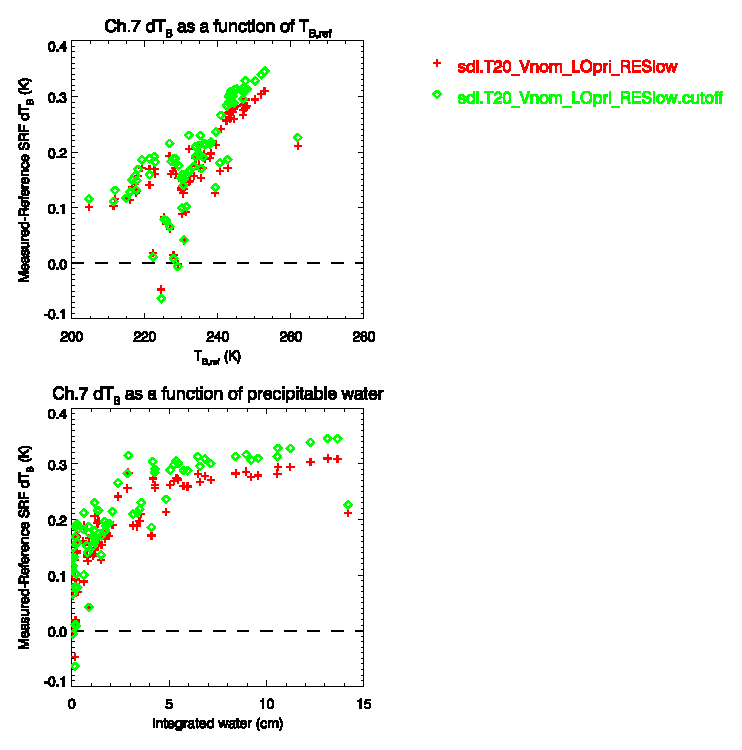
\includegraphics[bb=85 400 260 558,clip,scale=0.85]{graphics/dtb/Rset/e1.0_r0.0/atms_npp.ch7.dTb.eps} & 
    \includegraphics[bb=85 400 290 558,clip,scale=0.85]{graphics/dtb/Rset/e0.6_r0.4/atms_npp.ch7.dTb.eps} 
  \end{tabular} \\
  % the hand-crafted legend
  \setlength{\unitlength}{1cm}
  \begin{picture}(8.0,1.0)
    \thicklines
    \color{red}
    \put(-0.5,0.5){\line(1,0){1}}
    \put(0.7,0.35){\sffamily \textbf{+}\quad SRF wings included}
    \color{green}
    \put(5.0,0.5){\line(1,0){1}}
    \put(6.2,0.35){\sffamily {\Large$\diamond$}\quad SRF cutoff at -10dB}
  \end{picture}
  \caption{Channel 7 NPP ATMS nominal baseplate temperature (20\textdegree{}C) and bias voltage \textbf{(a)} SRF data digitized from the low spectral resolution plots in the ATMS PFM Calibration Data Book\cite{ATMS_PFM_CalLog} along with an SRF truncated at -10dB. The corresponding boxcar response based on table \ref{tab:atms_fo_sb_and_df} and a representative brightness temperature spectrum is also shown. \textbf{(b)} Brightness temperature differences showing the impact of excluding the SRF wings beyong -10dB, derived from MonoRTM calculations with a surface emissivity of unity. \textbf{(c)} Same as (b), but for surface emissivity and reflectivity of 0.6 and 0.4 respectively.}
  \label{fig:atms_npp.Rset.ch7}
\end{figure}
 
\begin{figure}[H]
  \centering
  \begin{tabular}{c c c}
    \textsf{\textbf{(a)} SRFs} &
    \textsf{\textbf{(b)} $\Delta T_B$ $(\epsilon_s = 1.0)$} &
    \textsf{\textbf{(c)} $\Delta T_B$ $(\epsilon_s = 0.6)$} \\
    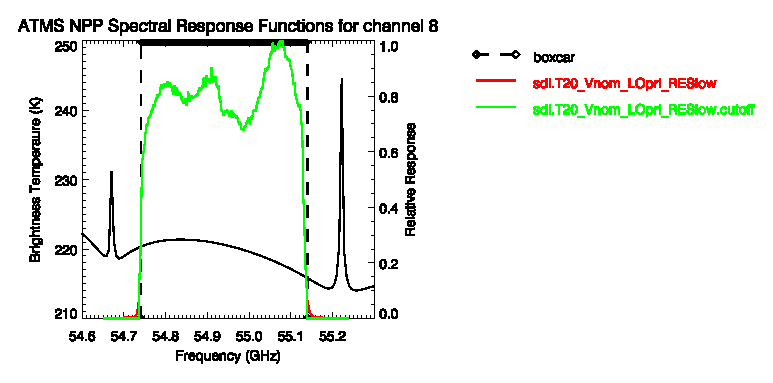
\includegraphics[bb=80 400 280 558,clip,scale=0.85]{graphics/srf/Rset/atms_npp.ch8.osrf.eps} &
    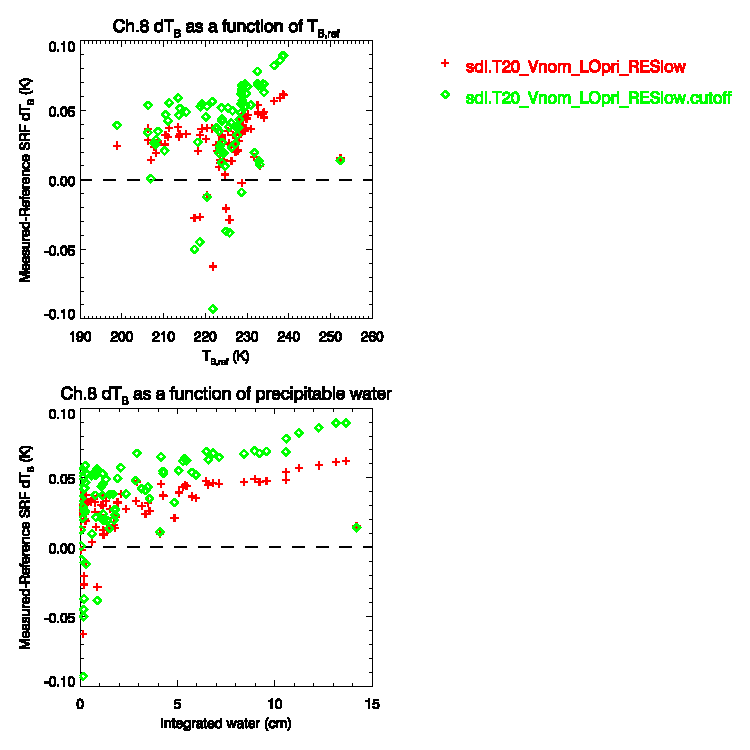
\includegraphics[bb=85 400 260 558,clip,scale=0.85]{graphics/dtb/Rset/e1.0_r0.0/atms_npp.ch8.dTb.eps} & 
    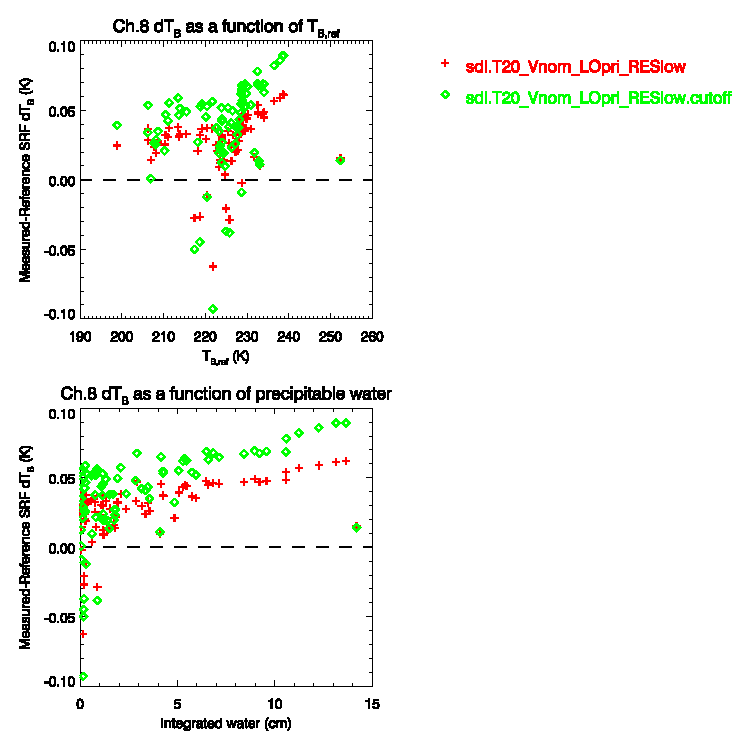
\includegraphics[bb=85 400 290 558,clip,scale=0.85]{graphics/dtb/Rset/e0.6_r0.4/atms_npp.ch8.dTb.eps} 
  \end{tabular} \\
  % the hand-crafted legend
  \setlength{\unitlength}{1cm}
  \begin{picture}(8.0,1.0)
    \thicklines
    \color{red}
    \put(-0.5,0.5){\line(1,0){1}}
    \put(0.7,0.35){\sffamily \textbf{+}\quad SRF wings included}
    \color{green}
    \put(5.0,0.5){\line(1,0){1}}
    \put(6.2,0.35){\sffamily {\Large$\diamond$}\quad SRF cutoff at -10dB}
  \end{picture}
  \caption{Channel 8 NPP ATMS nominal baseplate temperature (20\textdegree{}C) and bias voltage \textbf{(a)} SRF data digitized from the low spectral resolution plots in the ATMS PFM Calibration Data Book\cite{ATMS_PFM_CalLog} along with an SRF truncated at -10dB. The corresponding boxcar response based on table \ref{tab:atms_fo_sb_and_df} and a representative brightness temperature spectrum is also shown. \textbf{(b)} Brightness temperature differences showing the impact of excluding the SRF wings beyong -10dB, derived from MonoRTM calculations with a surface emissivity of unity. \textbf{(c)} Same as (b), but for surface emissivity and reflectivity of 0.6 and 0.4 respectively.}
  \label{fig:atms_npp.Rset.ch8}
\end{figure}
 
\begin{figure}[H]
  \centering
  \begin{tabular}{c c c}
    \textsf{\textbf{(a)} SRFs} &
    \textsf{\textbf{(b)} $\Delta T_B$ $(\epsilon_s = 1.0)$} &
    \textsf{\textbf{(c)} $\Delta T_B$ $(\epsilon_s = 0.6)$} \\
    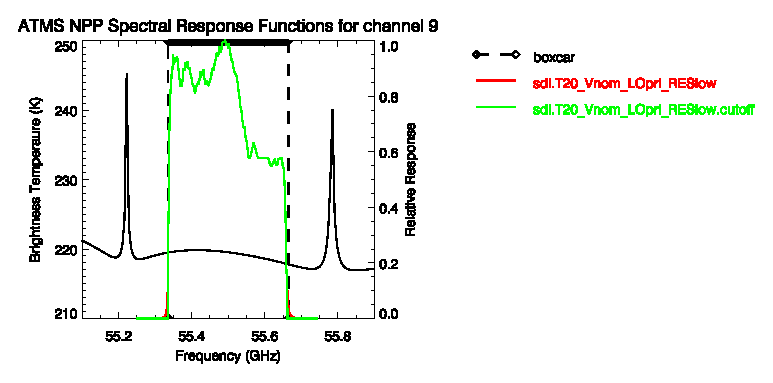
\includegraphics[bb=80 400 280 558,clip,scale=0.85]{graphics/srf/Rset/atms_npp.ch9.osrf.eps} &
    \includegraphics[bb=85 400 260 558,clip,scale=0.85]{graphics/dtb/Rset/e1.0_r0.0/atms_npp.ch9.dTb.eps} & 
    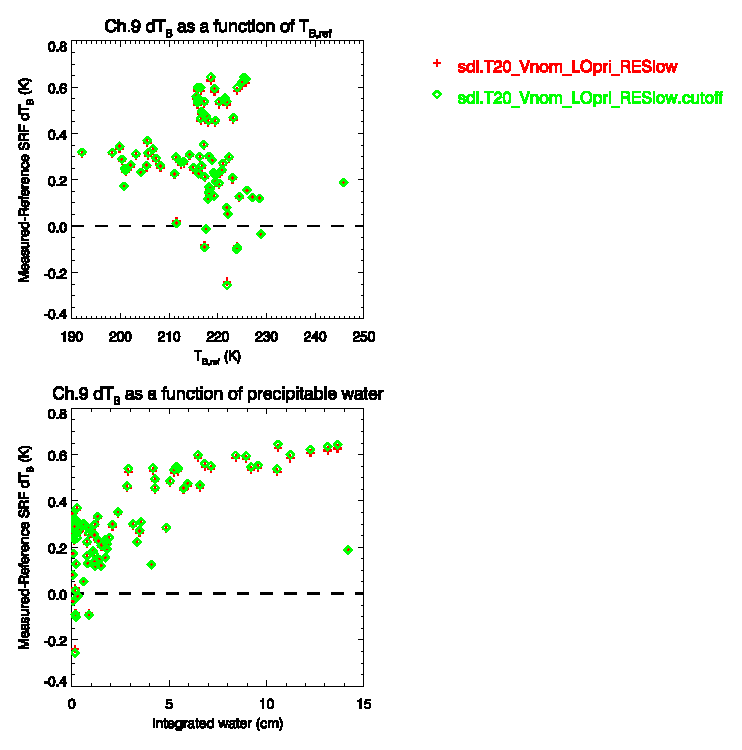
\includegraphics[bb=85 400 290 558,clip,scale=0.85]{graphics/dtb/Rset/e0.6_r0.4/atms_npp.ch9.dTb.eps} 
  \end{tabular} \\
  % the hand-crafted legend
  \setlength{\unitlength}{1cm}
  \begin{picture}(8.0,1.0)
    \thicklines
    \color{red}
    \put(-0.5,0.5){\line(1,0){1}}
    \put(0.7,0.35){\sffamily \textbf{+}\quad SRF wings included}
    \color{green}
    \put(5.0,0.5){\line(1,0){1}}
    \put(6.2,0.35){\sffamily {\Large$\diamond$}\quad SRF cutoff at -10dB}
  \end{picture}
  \caption{Channel 9 NPP ATMS nominal baseplate temperature (20\textdegree{}C) and bias voltage \textbf{(a)} SRF data digitized from the low spectral resolution plots in the ATMS PFM Calibration Data Book\cite{ATMS_PFM_CalLog} along with an SRF truncated at -10dB. The corresponding boxcar response based on table \ref{tab:atms_fo_sb_and_df} and a representative brightness temperature spectrum is also shown. \textbf{(b)} Brightness temperature differences showing the impact of excluding the SRF wings beyong -10dB, derived from MonoRTM calculations with a surface emissivity of unity. \textbf{(c)} Same as (b), but for surface emissivity and reflectivity of 0.6 and 0.4 respectively.}
  \label{fig:atms_npp.Rset.ch9}
\end{figure}
 
\begin{figure}[H]
  \centering
  \begin{tabular}{c c c}
    \textsf{\textbf{(a)} SRFs} &
    \textsf{\textbf{(b)} $\Delta T_B$ $(\epsilon_s = 1.0)$} &
    \textsf{\textbf{(c)} $\Delta T_B$ $(\epsilon_s = 0.6)$} \\
    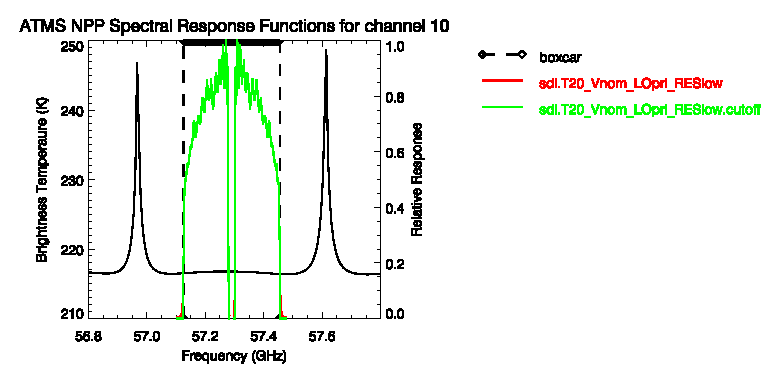
\includegraphics[bb=80 400 280 558,clip,scale=0.85]{graphics/srf/Rset/atms_npp.ch10.osrf.eps} &
    \includegraphics[bb=85 400 260 558,clip,scale=0.85]{graphics/dtb/Rset/e1.0_r0.0/atms_npp.ch10.dTb.eps} & 
    \includegraphics[bb=85 400 290 558,clip,scale=0.85]{graphics/dtb/Rset/e0.6_r0.4/atms_npp.ch10.dTb.eps} 
  \end{tabular} \\
  % the hand-crafted legend
  \setlength{\unitlength}{1cm}
  \begin{picture}(8.0,1.0)
    \thicklines
    \color{red}
    \put(-0.5,0.5){\line(1,0){1}}
    \put(0.7,0.35){\sffamily \textbf{+}\quad SRF wings included}
    \color{green}
    \put(5.0,0.5){\line(1,0){1}}
    \put(6.2,0.35){\sffamily {\Large$\diamond$}\quad SRF cutoff at -10dB}
  \end{picture}
  \caption{Channel 10 NPP ATMS nominal baseplate temperature (20\textdegree{}C) and bias voltage \textbf{(a)} SRF data digitized from the low spectral resolution plots in the ATMS PFM Calibration Data Book\cite{ATMS_PFM_CalLog} along with an SRF truncated at -10dB. The corresponding boxcar response based on table \ref{tab:atms_fo_sb_and_df} and a representative brightness temperature spectrum is also shown. \textbf{(b)} Brightness temperature differences showing the impact of excluding the SRF wings beyong -10dB, derived from MonoRTM calculations with a surface emissivity of unity. \textbf{(c)} Same as (b), but for surface emissivity and reflectivity of 0.6 and 0.4 respectively.}
  \label{fig:atms_npp.Rset.ch10}
\end{figure}
 
\begin{figure}[H]
  \centering
  \begin{tabular}{c c c}
    \textsf{\textbf{(a)} SRFs} &
    \textsf{\textbf{(b)} $\Delta T_B$ $(\epsilon_s = 1.0)$} &
    \textsf{\textbf{(c)} $\Delta T_B$ $(\epsilon_s = 0.6)$} \\
    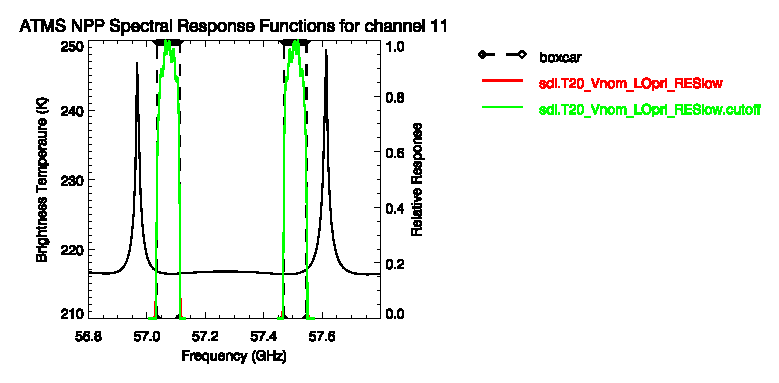
\includegraphics[bb=80 400 280 558,clip,scale=0.85]{graphics/srf/Rset/atms_npp.ch11.osrf.eps} &
    \includegraphics[bb=85 400 260 558,clip,scale=0.85]{graphics/dtb/Rset/e1.0_r0.0/atms_npp.ch11.dTb.eps} & 
    \includegraphics[bb=85 400 290 558,clip,scale=0.85]{graphics/dtb/Rset/e0.6_r0.4/atms_npp.ch11.dTb.eps} 
  \end{tabular} \\
  % the hand-crafted legend
  \setlength{\unitlength}{1cm}
  \begin{picture}(8.0,1.0)
    \thicklines
    \color{red}
    \put(-0.5,0.5){\line(1,0){1}}
    \put(0.7,0.35){\sffamily \textbf{+}\quad SRF wings included}
    \color{green}
    \put(5.0,0.5){\line(1,0){1}}
    \put(6.2,0.35){\sffamily {\Large$\diamond$}\quad SRF cutoff at -10dB}
  \end{picture}
  \caption{Channel 11 NPP ATMS nominal baseplate temperature (20\textdegree{}C) and bias voltage \textbf{(a)} SRF data digitized from the low spectral resolution plots in the ATMS PFM Calibration Data Book\cite{ATMS_PFM_CalLog} along with an SRF truncated at -10dB. The corresponding boxcar response based on table \ref{tab:atms_fo_sb_and_df} and a representative brightness temperature spectrum is also shown. \textbf{(b)} Brightness temperature differences showing the impact of excluding the SRF wings beyong -10dB, derived from MonoRTM calculations with a surface emissivity of unity. \textbf{(c)} Same as (b), but for surface emissivity and reflectivity of 0.6 and 0.4 respectively.}
  \label{fig:atms_npp.Rset.ch11}
\end{figure}
 
\begin{figure}[H]
  \centering
  \begin{tabular}{c c c}
    \textsf{\textbf{(a)} SRFs (low $f$ passbands only)} &
    \textsf{\textbf{(b)} $\Delta T_B$ $(\epsilon_s = 1.0)$} &
    \textsf{\textbf{(c)} $\Delta T_B$ $(\epsilon_s = 0.6)$} \\
    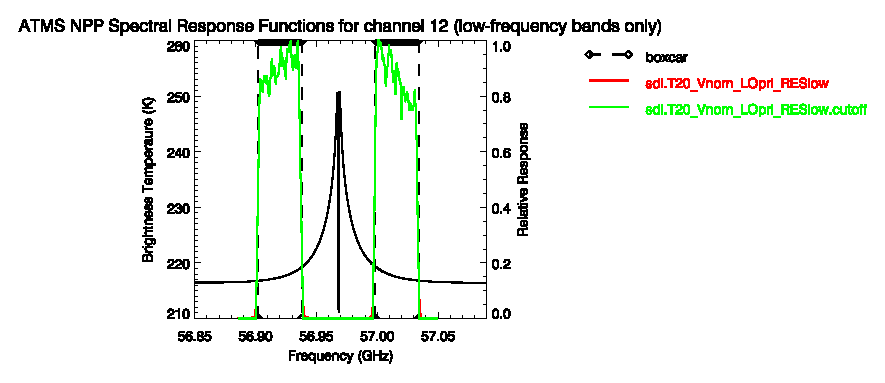
\includegraphics[bb=80 400 280 558,clip,scale=0.85]{graphics/srf/Rset/atms_npp.ch12.osrf.eps} &
    \includegraphics[bb=85 400 260 558,clip,scale=0.85]{graphics/dtb/Rset/e1.0_r0.0/atms_npp.ch12.dTb.eps} & 
    \includegraphics[bb=85 400 290 558,clip,scale=0.85]{graphics/dtb/Rset/e0.6_r0.4/atms_npp.ch12.dTb.eps} 
  \end{tabular} \\
  % the hand-crafted legend
  \setlength{\unitlength}{1cm}
  \begin{picture}(8.0,1.0)
    \thicklines
    \color{red}
    \put(-0.5,0.5){\line(1,0){1}}
    \put(0.7,0.35){\sffamily \textbf{+}\quad SRF wings included}
    \color{green}
    \put(5.0,0.5){\line(1,0){1}}
    \put(6.2,0.35){\sffamily {\Large$\diamond$}\quad SRF cutoff at -10dB}
  \end{picture}
  \caption{Channel 12 NPP ATMS nominal baseplate temperature (20\textdegree{}C) and bias voltage \textbf{(a)} SRF data digitized from the low spectral resolution plots in the ATMS PFM Calibration Data Book\cite{ATMS_PFM_CalLog} along with an SRF truncated at -10dB. The corresponding boxcar response based on table \ref{tab:atms_fo_sb_and_df} and a representative brightness temperature spectrum is also shown. \textbf{(b)} Brightness temperature differences showing the impact of excluding the SRF wings beyong -10dB, derived from MonoRTM calculations with a surface emissivity of unity. \textbf{(c)} Same as (b), but for surface emissivity and reflectivity of 0.6 and 0.4 respectively.}
  \label{fig:atms_npp.Rset.ch12}
\end{figure}
 
\begin{figure}[H]
  \centering
  \begin{tabular}{c c c}
    \textsf{\textbf{(a)} SRFs (low $f$ passbands only)} &
    \textsf{\textbf{(b)} $\Delta T_B$ $(\epsilon_s = 1.0)$} &
    \textsf{\textbf{(c)} $\Delta T_B$ $(\epsilon_s = 0.6)$} \\
    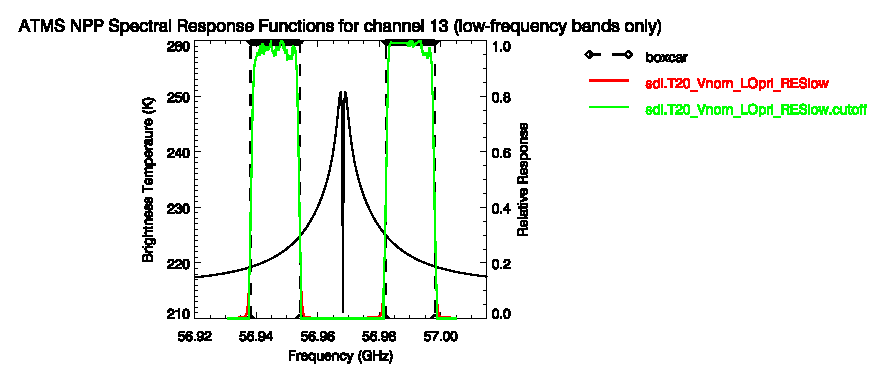
\includegraphics[bb=80 400 280 558,clip,scale=0.85]{graphics/srf/Rset/atms_npp.ch13.osrf.eps} &
    \includegraphics[bb=85 400 260 558,clip,scale=0.85]{graphics/dtb/Rset/e1.0_r0.0/atms_npp.ch13.dTb.eps} & 
    \includegraphics[bb=85 400 290 558,clip,scale=0.85]{graphics/dtb/Rset/e0.6_r0.4/atms_npp.ch13.dTb.eps} 
  \end{tabular} \\
  % the hand-crafted legend
  \setlength{\unitlength}{1cm}
  \begin{picture}(8.0,1.0)
    \thicklines
    \color{red}
    \put(-0.5,0.5){\line(1,0){1}}
    \put(0.7,0.35){\sffamily \textbf{+}\quad SRF wings included}
    \color{green}
    \put(5.0,0.5){\line(1,0){1}}
    \put(6.2,0.35){\sffamily {\Large$\diamond$}\quad SRF cutoff at -10dB}
  \end{picture}
  \caption{Channel 13 NPP ATMS nominal baseplate temperature (20\textdegree{}C) and bias voltage \textbf{(a)} SRF data digitized from the low spectral resolution plots in the ATMS PFM Calibration Data Book\cite{ATMS_PFM_CalLog} along with an SRF truncated at -10dB. The corresponding boxcar response based on table \ref{tab:atms_fo_sb_and_df} and a representative brightness temperature spectrum is also shown. \textbf{(b)} Brightness temperature differences showing the impact of excluding the SRF wings beyong -10dB, derived from MonoRTM calculations with a surface emissivity of unity. \textbf{(c)} Same as (b), but for surface emissivity and reflectivity of 0.6 and 0.4 respectively.}
  \label{fig:atms_npp.Rset.ch13}
\end{figure}
 
\begin{figure}[H]
  \centering
  \begin{tabular}{c c c}
    \textsf{\textbf{(a)} SRFs (low $f$ passbands only)} &
    \textsf{\textbf{(b)} $\Delta T_B$ $(\epsilon_s = 1.0)$} &
    \textsf{\textbf{(c)} $\Delta T_B$ $(\epsilon_s = 0.6)$} \\
    \includegraphics[bb=80 400 280 558,clip,scale=0.85]{graphics/srf/Rset/atms_npp.ch14.osrf.eps} &
    \includegraphics[bb=85 400 260 558,clip,scale=0.85]{graphics/dtb/Rset/e1.0_r0.0/atms_npp.ch14.dTb.eps} & 
    \includegraphics[bb=85 400 290 558,clip,scale=0.85]{graphics/dtb/Rset/e0.6_r0.4/atms_npp.ch14.dTb.eps} 
  \end{tabular} \\
  % the hand-crafted legend
  \setlength{\unitlength}{1cm}
  \begin{picture}(8.0,1.0)
    \thicklines
    \color{red}
    \put(-0.5,0.5){\line(1,0){1}}
    \put(0.7,0.35){\sffamily \textbf{+}\quad SRF wings included}
    \color{green}
    \put(5.0,0.5){\line(1,0){1}}
    \put(6.2,0.35){\sffamily {\Large$\diamond$}\quad SRF cutoff at -10dB}
  \end{picture}
  \caption{Channel 14 NPP ATMS nominal baseplate temperature (20\textdegree{}C) and bias voltage \textbf{(a)} SRF data digitized from the low spectral resolution plots in the ATMS PFM Calibration Data Book\cite{ATMS_PFM_CalLog} along with an SRF truncated at -10dB. The corresponding boxcar response based on table \ref{tab:atms_fo_sb_and_df} and a representative brightness temperature spectrum is also shown. \textbf{(b)} Brightness temperature differences showing the impact of excluding the SRF wings beyong -10dB, derived from MonoRTM calculations with a surface emissivity of unity. \textbf{(c)} Same as (b), but for surface emissivity and reflectivity of 0.6 and 0.4 respectively.}
  \label{fig:atms_npp.Rset.ch14}
\end{figure}
 
\begin{figure}[H]
  \centering
  \begin{tabular}{c c c}
    \textsf{\textbf{(a)} SRFs (low $f$ passbands only)} &
    \textsf{\textbf{(b)} $\Delta T_B$ $(\epsilon_s = 1.0)$} &
    \textsf{\textbf{(c)} $\Delta T_B$ $(\epsilon_s = 0.6)$} \\
    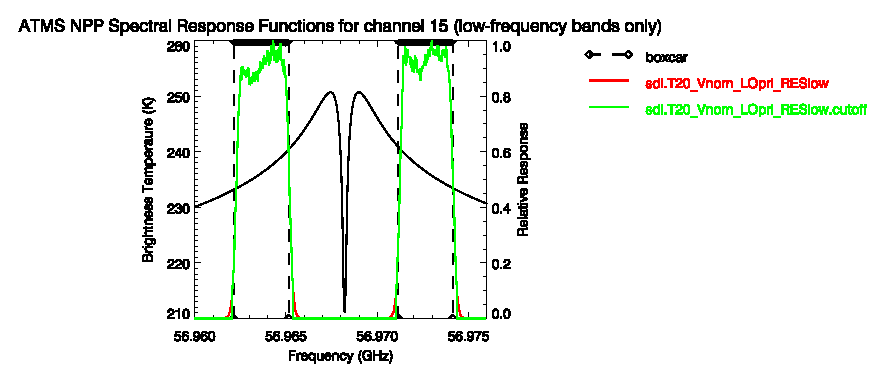
\includegraphics[bb=80 400 280 558,clip,scale=0.85]{graphics/srf/Rset/atms_npp.ch15.osrf.eps} &
    \includegraphics[bb=85 400 260 558,clip,scale=0.85]{graphics/dtb/Rset/e1.0_r0.0/atms_npp.ch15.dTb.eps} & 
    \includegraphics[bb=85 400 290 558,clip,scale=0.85]{graphics/dtb/Rset/e0.6_r0.4/atms_npp.ch15.dTb.eps} 
  \end{tabular} \\
  % the hand-crafted legend
  \setlength{\unitlength}{1cm}
  \begin{picture}(8.0,1.0)
    \thicklines
    \color{red}
    \put(-0.5,0.5){\line(1,0){1}}
    \put(0.7,0.35){\sffamily \textbf{+}\quad SRF wings included}
    \color{green}
    \put(5.0,0.5){\line(1,0){1}}
    \put(6.2,0.35){\sffamily {\Large$\diamond$}\quad SRF cutoff at -10dB}
  \end{picture}
  \caption{Channel 15 NPP ATMS nominal baseplate temperature (20\textdegree{}C) and bias voltage \textbf{(a)} SRF data digitized from the low spectral resolution plots in the ATMS PFM Calibration Data Book\cite{ATMS_PFM_CalLog} along with an SRF truncated at -10dB. The corresponding boxcar response based on table \ref{tab:atms_fo_sb_and_df} and a representative brightness temperature spectrum is also shown. \textbf{(b)} Brightness temperature differences showing the impact of excluding the SRF wings beyong -10dB, derived from MonoRTM calculations with a surface emissivity of unity. \textbf{(c)} Same as (b), but for surface emissivity and reflectivity of 0.6 and 0.4 respectively.}
  \label{fig:atms_npp.Rset.ch15}
\end{figure}
 
\begin{figure}[H]
  \centering
  \begin{tabular}{c c c}
    \textsf{\textbf{(a)} SRFs} &
    \textsf{\textbf{(b)} $\Delta T_B$ $(\epsilon_s = 1.0)$} &
    \textsf{\textbf{(c)} $\Delta T_B$ $(\epsilon_s = 0.6)$} \\
    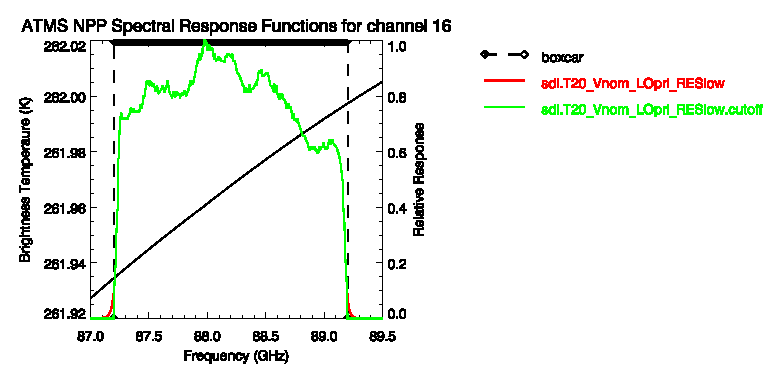
\includegraphics[bb=80 400 280 558,clip,scale=0.85]{graphics/srf/Rset/atms_npp.ch16.osrf.eps} &
    \includegraphics[bb=85 400 260 558,clip,scale=0.85]{graphics/dtb/Rset/e1.0_r0.0/atms_npp.ch16.dTb.eps} & 
    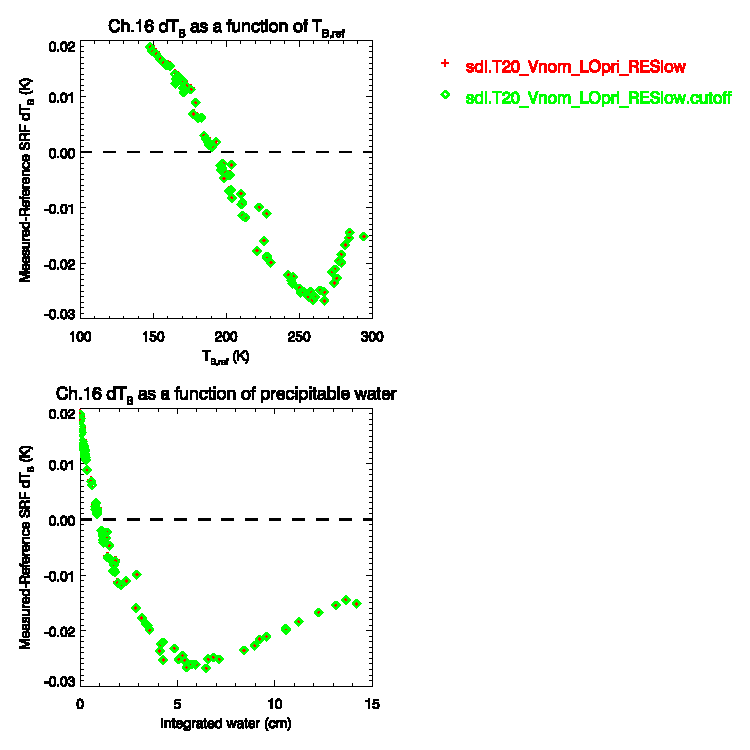
\includegraphics[bb=85 400 290 558,clip,scale=0.85]{graphics/dtb/Rset/e0.6_r0.4/atms_npp.ch16.dTb.eps} 
  \end{tabular} \\
  % the hand-crafted legend
  \setlength{\unitlength}{1cm}
  \begin{picture}(8.0,1.0)
    \thicklines
    \color{red}
    \put(-0.5,0.5){\line(1,0){1}}
    \put(0.7,0.35){\sffamily \textbf{+}\quad SRF wings included}
    \color{green}
    \put(5.0,0.5){\line(1,0){1}}
    \put(6.2,0.35){\sffamily {\Large$\diamond$}\quad SRF cutoff at -10dB}
  \end{picture}
  \caption{Channel 16 NPP ATMS nominal baseplate temperature (20\textdegree{}C) and bias voltage \textbf{(a)} SRF data digitized from the low spectral resolution plots in the ATMS PFM Calibration Data Book\cite{ATMS_PFM_CalLog} along with an SRF truncated at -10dB. The corresponding boxcar response based on table \ref{tab:atms_fo_sb_and_df} and a representative brightness temperature spectrum is also shown. \textbf{(b)} Brightness temperature differences showing the impact of excluding the SRF wings beyong -10dB, derived from MonoRTM calculations with a surface emissivity of unity. \textbf{(c)} Same as (b), but for surface emissivity and reflectivity of 0.6 and 0.4 respectively.}
  \label{fig:atms_npp.Rset.ch16}
\end{figure}
 
\begin{figure}[H]
  \centering
  \begin{tabular}{c c c}
    \textsf{\textbf{(a)} SRFs} &
    \textsf{\textbf{(b)} $\Delta T_B$ $(\epsilon_s = 1.0)$} &
    \textsf{\textbf{(c)} $\Delta T_B$ $(\epsilon_s = 0.6)$} \\
    \includegraphics[bb=80 400 280 558,clip,scale=0.85]{graphics/srf/Rset/atms_npp.ch17.osrf.eps} &
    \includegraphics[bb=85 400 260 558,clip,scale=0.85]{graphics/dtb/Rset/e1.0_r0.0/atms_npp.ch17.dTb.eps} & 
    \includegraphics[bb=85 400 290 558,clip,scale=0.85]{graphics/dtb/Rset/e0.6_r0.4/atms_npp.ch17.dTb.eps} 
  \end{tabular} \\
  % the hand-crafted legend
  \setlength{\unitlength}{1cm}
  \begin{picture}(8.0,1.0)
    \thicklines
    \color{red}
    \put(-0.5,0.5){\line(1,0){1}}
    \put(0.7,0.35){\sffamily \textbf{+}\quad SRF wings included}
    \color{green}
    \put(5.0,0.5){\line(1,0){1}}
    \put(6.2,0.35){\sffamily {\Large$\diamond$}\quad SRF cutoff at -10dB}
  \end{picture}
  \caption{Channel 17 NPP ATMS nominal baseplate temperature (20\textdegree{}C) and bias voltage \textbf{(a)} SRF data digitized from the low spectral resolution plots in the ATMS PFM Calibration Data Book\cite{ATMS_PFM_CalLog} along with an SRF truncated at -10dB. The corresponding boxcar response based on table \ref{tab:atms_fo_sb_and_df} and a representative brightness temperature spectrum is also shown. \textbf{(b)} Brightness temperature differences showing the impact of excluding the SRF wings beyong -10dB, derived from MonoRTM calculations with a surface emissivity of unity. \textbf{(c)} Same as (b), but for surface emissivity and reflectivity of 0.6 and 0.4 respectively.}
  \label{fig:atms_npp.Rset.ch17}
\end{figure}
 
\begin{figure}[H]
  \centering
  \begin{tabular}{c c c}
    \textsf{\textbf{(a)} SRFs} &
    \textsf{\textbf{(b)} $\Delta T_B$ $(\epsilon_s = 1.0)$} &
    \textsf{\textbf{(c)} $\Delta T_B$ $(\epsilon_s = 0.6)$} \\
    \includegraphics[bb=80 400 280 558,clip,scale=0.85]{graphics/srf/Rset/atms_npp.ch18.osrf.eps} &
    \includegraphics[bb=85 400 260 558,clip,scale=0.85]{graphics/dtb/Rset/e1.0_r0.0/atms_npp.ch18.dTb.eps} & 
    \includegraphics[bb=85 400 290 558,clip,scale=0.85]{graphics/dtb/Rset/e0.6_r0.4/atms_npp.ch18.dTb.eps} 
  \end{tabular} \\
  % the hand-crafted legend
  \setlength{\unitlength}{1cm}
  \begin{picture}(8.0,1.0)
    \thicklines
    \color{red}
    \put(-0.5,0.5){\line(1,0){1}}
    \put(0.7,0.35){\sffamily \textbf{+}\quad SRF wings included}
    \color{green}
    \put(5.0,0.5){\line(1,0){1}}
    \put(6.2,0.35){\sffamily {\Large$\diamond$}\quad SRF cutoff at -10dB}
  \end{picture}
  \caption{Channel 18 NPP ATMS nominal baseplate temperature (20\textdegree{}C) and bias voltage \textbf{(a)} SRF data digitized from the low spectral resolution plots in the ATMS PFM Calibration Data Book\cite{ATMS_PFM_CalLog} along with an SRF truncated at -10dB. The corresponding boxcar response based on table \ref{tab:atms_fo_sb_and_df} and a representative brightness temperature spectrum is also shown. \textbf{(b)} Brightness temperature differences showing the impact of excluding the SRF wings beyong -10dB, derived from MonoRTM calculations with a surface emissivity of unity. \textbf{(c)} Same as (b), but for surface emissivity and reflectivity of 0.6 and 0.4 respectively.}
  \label{fig:atms_npp.Rset.ch18}
\end{figure}
 
\begin{figure}[H]
  \centering
  \begin{tabular}{c c c}
    \textsf{\textbf{(a)} SRFs} &
    \textsf{\textbf{(b)} $\Delta T_B$ $(\epsilon_s = 1.0)$} &
    \textsf{\textbf{(c)} $\Delta T_B$ $(\epsilon_s = 0.6)$} \\
    \includegraphics[bb=80 400 280 558,clip,scale=0.85]{graphics/srf/Rset/atms_npp.ch19.osrf.eps} &
    \includegraphics[bb=85 400 260 558,clip,scale=0.85]{graphics/dtb/Rset/e1.0_r0.0/atms_npp.ch19.dTb.eps} & 
    \includegraphics[bb=85 400 290 558,clip,scale=0.85]{graphics/dtb/Rset/e0.6_r0.4/atms_npp.ch19.dTb.eps} 
  \end{tabular} \\
  % the hand-crafted legend
  \setlength{\unitlength}{1cm}
  \begin{picture}(8.0,1.0)
    \thicklines
    \color{red}
    \put(-0.5,0.5){\line(1,0){1}}
    \put(0.7,0.35){\sffamily \textbf{+}\quad SRF wings included}
    \color{green}
    \put(5.0,0.5){\line(1,0){1}}
    \put(6.2,0.35){\sffamily {\Large$\diamond$}\quad SRF cutoff at -10dB}
  \end{picture}
  \caption{Channel 19 NPP ATMS nominal baseplate temperature (20\textdegree{}C) and bias voltage \textbf{(a)} SRF data digitized from the low spectral resolution plots in the ATMS PFM Calibration Data Book\cite{ATMS_PFM_CalLog} along with an SRF truncated at -10dB. The corresponding boxcar response based on table \ref{tab:atms_fo_sb_and_df} and a representative brightness temperature spectrum is also shown. \textbf{(b)} Brightness temperature differences showing the impact of excluding the SRF wings beyong -10dB, derived from MonoRTM calculations with a surface emissivity of unity. \textbf{(c)} Same as (b), but for surface emissivity and reflectivity of 0.6 and 0.4 respectively.}
  \label{fig:atms_npp.Rset.ch19}
\end{figure}
 
\begin{figure}[H]
  \centering
  \begin{tabular}{c c c}
    \textsf{\textbf{(a)} SRFs} &
    \textsf{\textbf{(b)} $\Delta T_B$ $(\epsilon_s = 1.0)$} &
    \textsf{\textbf{(c)} $\Delta T_B$ $(\epsilon_s = 0.6)$} \\
    \includegraphics[bb=80 400 280 558,clip,scale=0.85]{graphics/srf/Rset/atms_npp.ch20.osrf.eps} &
    \includegraphics[bb=85 400 260 558,clip,scale=0.85]{graphics/dtb/Rset/e1.0_r0.0/atms_npp.ch20.dTb.eps} & 
    \includegraphics[bb=85 400 290 558,clip,scale=0.85]{graphics/dtb/Rset/e0.6_r0.4/atms_npp.ch20.dTb.eps} 
  \end{tabular} \\
  % the hand-crafted legend
  \setlength{\unitlength}{1cm}
  \begin{picture}(8.0,1.0)
    \thicklines
    \color{red}
    \put(-0.5,0.5){\line(1,0){1}}
    \put(0.7,0.35){\sffamily \textbf{+}\quad SRF wings included}
    \color{green}
    \put(5.0,0.5){\line(1,0){1}}
    \put(6.2,0.35){\sffamily {\Large$\diamond$}\quad SRF cutoff at -10dB}
  \end{picture}
  \caption{Channel 20 NPP ATMS nominal baseplate temperature (20\textdegree{}C) and bias voltage \textbf{(a)} SRF data digitized from the low spectral resolution plots in the ATMS PFM Calibration Data Book\cite{ATMS_PFM_CalLog} along with an SRF truncated at -10dB. The corresponding boxcar response based on table \ref{tab:atms_fo_sb_and_df} and a representative brightness temperature spectrum is also shown. \textbf{(b)} Brightness temperature differences showing the impact of excluding the SRF wings beyong -10dB, derived from MonoRTM calculations with a surface emissivity of unity. \textbf{(c)} Same as (b), but for surface emissivity and reflectivity of 0.6 and 0.4 respectively.}
  \label{fig:atms_npp.Rset.ch20}
\end{figure}
 
\begin{figure}[H]
  \centering
  \begin{tabular}{c c c}
    \textsf{\textbf{(a)} SRFs} &
    \textsf{\textbf{(b)} $\Delta T_B$ $(\epsilon_s = 1.0)$} &
    \textsf{\textbf{(c)} $\Delta T_B$ $(\epsilon_s = 0.6)$} \\
    \includegraphics[bb=80 400 280 558,clip,scale=0.85]{graphics/srf/Rset/atms_npp.ch21.osrf.eps} &
    \includegraphics[bb=85 400 260 558,clip,scale=0.85]{graphics/dtb/Rset/e1.0_r0.0/atms_npp.ch21.dTb.eps} & 
    \includegraphics[bb=85 400 290 558,clip,scale=0.85]{graphics/dtb/Rset/e0.6_r0.4/atms_npp.ch21.dTb.eps} 
  \end{tabular} \\
  % the hand-crafted legend
  \setlength{\unitlength}{1cm}
  \begin{picture}(8.0,1.0)
    \thicklines
    \color{red}
    \put(-0.5,0.5){\line(1,0){1}}
    \put(0.7,0.35){\sffamily \textbf{+}\quad SRF wings included}
    \color{green}
    \put(5.0,0.5){\line(1,0){1}}
    \put(6.2,0.35){\sffamily {\Large$\diamond$}\quad SRF cutoff at -10dB}
  \end{picture}
  \caption{Channel 21 NPP ATMS nominal baseplate temperature (20\textdegree{}C) and bias voltage \textbf{(a)} SRF data digitized from the low spectral resolution plots in the ATMS PFM Calibration Data Book\cite{ATMS_PFM_CalLog} along with an SRF truncated at -10dB. The corresponding boxcar response based on table \ref{tab:atms_fo_sb_and_df} and a representative brightness temperature spectrum is also shown. \textbf{(b)} Brightness temperature differences showing the impact of excluding the SRF wings beyong -10dB, derived from MonoRTM calculations with a surface emissivity of unity. \textbf{(c)} Same as (b), but for surface emissivity and reflectivity of 0.6 and 0.4 respectively.}
  \label{fig:atms_npp.Rset.ch21}
\end{figure}
 
\begin{figure}[H]
  \centering
  \begin{tabular}{c c c}
    \textsf{\textbf{(a)} SRFs} &
    \textsf{\textbf{(b)} $\Delta T_B$ $(\epsilon_s = 1.0)$} &
    \textsf{\textbf{(c)} $\Delta T_B$ $(\epsilon_s = 0.6)$} \\
    \includegraphics[bb=80 400 280 558,clip,scale=0.85]{graphics/srf/Rset/atms_npp.ch22.osrf.eps} &
    \includegraphics[bb=85 400 260 558,clip,scale=0.85]{graphics/dtb/Rset/e1.0_r0.0/atms_npp.ch22.dTb.eps} & 
    \includegraphics[bb=85 400 290 558,clip,scale=0.85]{graphics/dtb/Rset/e0.6_r0.4/atms_npp.ch22.dTb.eps} 
  \end{tabular} \\
  % the hand-crafted legend
  \setlength{\unitlength}{1cm}
  \begin{picture}(8.0,1.0)
    \thicklines
    \color{red}
    \put(-0.5,0.5){\line(1,0){1}}
    \put(0.7,0.35){\sffamily \textbf{+}\quad SRF wings included}
    \color{green}
    \put(5.0,0.5){\line(1,0){1}}
    \put(6.2,0.35){\sffamily {\Large$\diamond$}\quad SRF cutoff at -10dB}
  \end{picture}
  \caption{Channel 22 NPP ATMS nominal baseplate temperature (20\textdegree{}C) and bias voltage \textbf{(a)} SRF data digitized from the low spectral resolution plots in the ATMS PFM Calibration Data Book\cite{ATMS_PFM_CalLog} along with an SRF truncated at -10dB. The corresponding boxcar response based on table \ref{tab:atms_fo_sb_and_df} and a representative brightness temperature spectrum is also shown. \textbf{(b)} Brightness temperature differences showing the impact of excluding the SRF wings beyong -10dB, derived from MonoRTM calculations with a surface emissivity of unity. \textbf{(c)} Same as (b), but for surface emissivity and reflectivity of 0.6 and 0.4 respectively.}
  \label{fig:atms_npp.Rset.ch22}
\end{figure}
 
